\section{Conclusiones y trabajos futuros}
\subsection{Conclusiones}

\begin{frame}
  \frametitle{Conclusiones}
  \begin{enumerate}
    \item \textbf{Primer método} que estima la calidad de reconstrucciones biomédicas 3D.
    \item Se logra generar un \textbf{conjunto de datos sintéticos médicos} para estimación de calidad.
    \item \textbf{Se justifica} el uso de modelos de \textbf{aprendizaje profundo} \alert{experimentalmente}.
    \item Pese a ser un estudio preliminar, obtenemos una \textbf{alta correlación (88\%)}. Indicador 
      de lo prometedora que es esta línea de investigación.
  \end{enumerate}
\end{frame}

\begin{frame}
    \frametitle{Conclusiones}
\begin{figure}
  \vspace{-.5cm}
  \hspace{-.2cm}\subfloat[Submuestreo al 10\%]{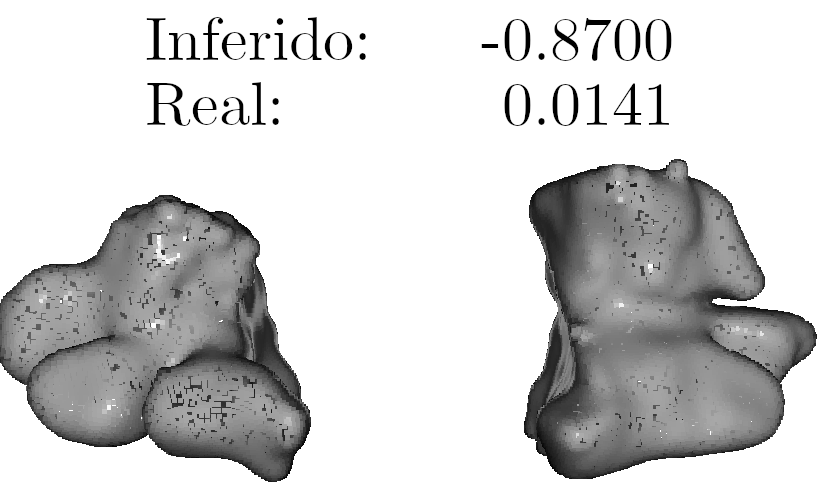
\includegraphics[width=.3\textwidth]{imagenes/chapter5/Maxiliar100014_7.png}}\hspace{.2cm}
  \subfloat[Submuestreo al 30\%]{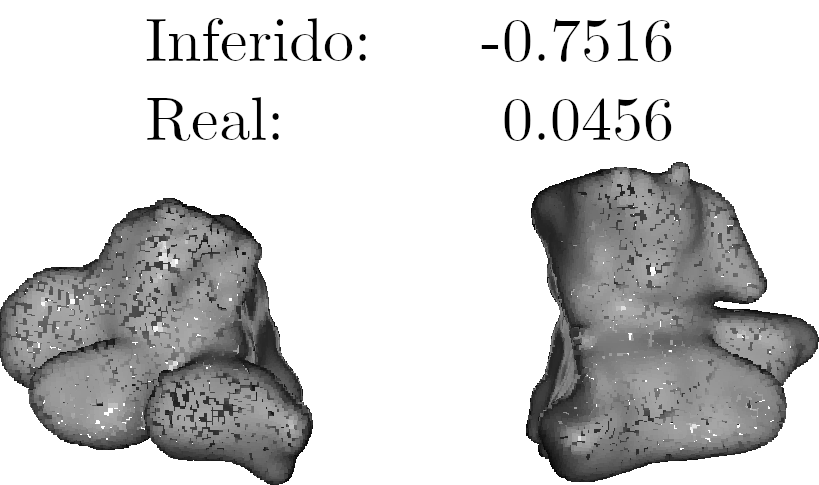
\includegraphics[width=.3\textwidth]{imagenes/chapter5/Maxiliar100014_9.png}}\hspace{.2cm}
  \subfloat[Submuestreo al 60\%]{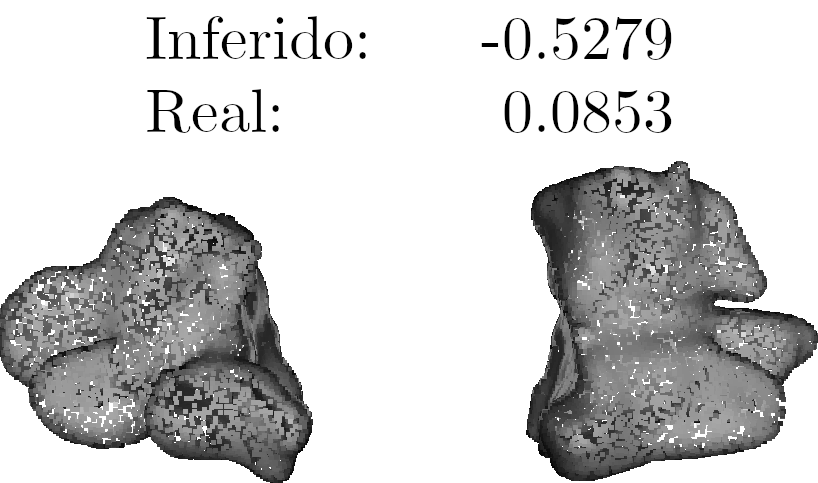
\includegraphics[width=.3\textwidth]{imagenes/chapter5/Maxiliar100014_11.png}}
  \caption{Ejemplo de correspondencia de pendiente entre valores inferidos (sin normalizar) y 
  los valores reales de las etiquetas.} 
  \label{fig:Cualitativos}
\end{figure}
\vspace{-.5cm}
\begin{enumerate}
  \item Se han completado satisfactoriamente los objetivos planteados.
  \item Se han abierto puertas a futuras investigaciones.
  \item \url{https://github.com/CodeBoy-source/TFG_NRPCQA} 
\end{enumerate}
\end{frame}

\begin{frame}
  \frametitle{Trabajos futuros}
  \begin{enumerate}
    \item Rehacer el experimento con \textbf{etiquetas generadas manualmente}. 
    \item \textbf{Para mejorar el meta-modelo}, se podria \alert{permitir la adaptación} del modelo de extracción de características \textbf{temporales}.
    \item Simular distorsiones sobre \textbf{imágenes 2D} para obtener datos más \textbf{realistas}.
    \item Explorar \alert{otros métodos} de la literatura. 
  \end{enumerate}
\end{frame}


